% Based on a TeXnicCenter-Template by Gyorgy SZEIDL.
%%%%%%%%%%%%%%%%%%%%%%%%%%%%%%%%%%%%%%%%%%%%%%%%%%%%%%%%%%%%%

%------------------------------------------------------------
%
\documentclass[a4paper]{article}%
%Options -- Point size: 10pt (default), 11pt, 12pt
% -- Paper size: letterpaper (default), a4paper, a5paper, b5paper
% legalpaper, executivepaper
% -- Orientation (portrait is the default)
% landscape
% -- Print size: oneside (default), twoside
% -- Quality final(default), draft
% -- Title page notitlepage, titlepage(default)
% -- Columns onecolumn(default), twocolumn
% -- Equation numbering (equation numbers on the right is the default)
% leqno
% -- Displayed equations (centered is the default)
% fleqn (equations start at the same distance from the right side)
% -- Open bibliography style (closed is the default)
% openbib
% For instance the command
% \documentclass[a4paper,12pt,leqno]{article}
% ensures that the paper size is a4, the fonts are typeset at the size 12p
% and the equation numbers are on the left side
%
\usepackage{amsmath}%
\usepackage{amsfonts}%
\usepackage{amssymb}%
\usepackage{graphicx}

\usepackage[utf8]{inputenc}
\usepackage[T1]{fontenc}
\usepackage[francais]{babel}
\usepackage{float}
%\usepackage[pdftex]{graphicx}
\usepackage[colorinlistoftodos]{todonotes}


%-------------------------------------------

\newcommand{\HRule}{\rule{\linewidth}{0.27mm}}

\begin{document}

\begin{titlepage}
\begin{center}

% Upper part of the page. The '~' is needed because \\
% only works if a paragraph has started.
\begin{flushleft}

\includegraphics[width=0.5\textwidth]{./images/LogotypeINSARennes-web-RVB.png}~\\[1cm]
\end{flushleft}

% Title
\textsc{\LARGE Jeu Small World}\\
\huge \bfseries Rapport de conception \\[1cm]

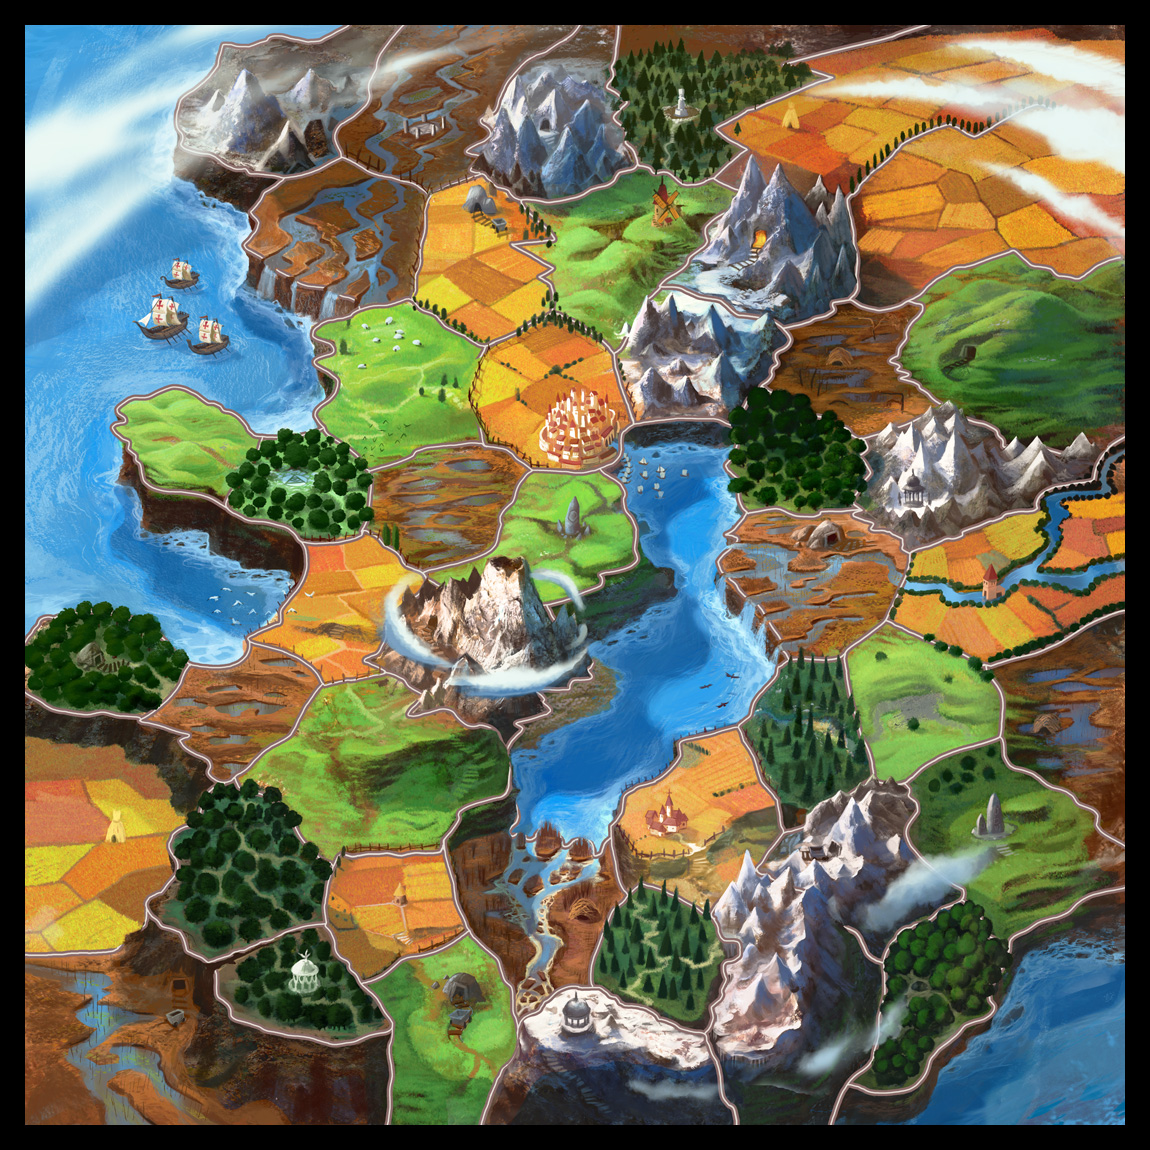
\includegraphics[width=0.8\textwidth]{./images/plateau_smallworld.jpg}~\\[1cm]


% Author and supervisor
\begin{minipage}{0.4\textwidth}
\begin{flushleft} \large
\emph{Auteurs :}\\
Fabien \textsc{Dubar}\\
Tom \textsc{Demulier--Chevret}\\
\end{flushleft}
\end{minipage}
\begin{minipage}{0.4\textwidth}
\begin{flushright} \large
\emph{Enseignants :} \\
Eric \textsc{Anquetil}\\
Arnaud \textsc{Blouin}\\
Manuel \textsc{Bouillon}\\
Grégoire \textsc{Richard}\\
Maud \textsc{Marchal}\\
\end{flushright}
\end{minipage}

\vfill


\end{center}
\end{titlepage}


\newpage

~
\newpage

\tableofcontents

\newpage
~
\newpage

\section*{Introduction}
\addcontentsline{toc}{section}{Introduction}

L'objectif du projet d'analyse, conception et POO de quatrième année informatique est la création d'un jeu vidéo basé sur le jeu de plateau Small World, pour mettre en pratique et appliquer les concepts vu en cours de modélisation et POO.

\medskip

SmallWorld est un jeu de plateau tour par tour dans lequel chaque joueur dirige un peuple sur une carte composée de cases. Chaque peuple comporte plusieurs unités disposées sur dans sur la carte, que le joueur peut choisir de déplacer ou de faire combattre.
Chaque unité rapporte un certains nombre de points par tour à son propriétaire. 
Le joueur gagnant est celui ayant amassé le plus de point en fin de partie.

\medskip

Vous pouvez retrouver les règles complètes du jeu dans le polycopié de sujet du projet ainsi que sur les forums (des modifications ayant été apportées depuis le départ).

\medskip

Ce rapport fait état de nos choix de conception et modélisation à travers les diagrammes de classes, de séquence, d'activité et d'état-transition, ainsi que leur explications (notamment pour l'utilisation de certains patrons de conception).

De cette phase d'analyse et de conception découlera la phase d'implémentation.

\medskip

Tous les diagrammes cités dans ce rapport se retrouvent aussi dans le dossier ./images de l'archive contenant ce rapport.

\newpage

\section{Analyse}


\subsection{Création d'une partie}

Dans le jeu SmallWorld, le Maitre du Jeu a la possibilité de créer une partie selon le type qui lui convient : une partie très courte (type Démo), Petite ou Normale. Cela impacte la taille de la carte, le nombre d'unité disponibles ainsi que le nombre de tour à jouer. De plus, les deux Joueurs peuvent avoir la possibilité de choisir le peuple qu'ils désirent.
Nous retrouvons ces fonctionnalités sur le diagramme de cas d'usages Figure~\ref{fig:use_case_creationpartie} ainsi que les les interactions entre objets sur le diagramme de sequence Figure~\ref{fig:sequence_creationpartie}.


\begin{figure}[H]
    \centering
    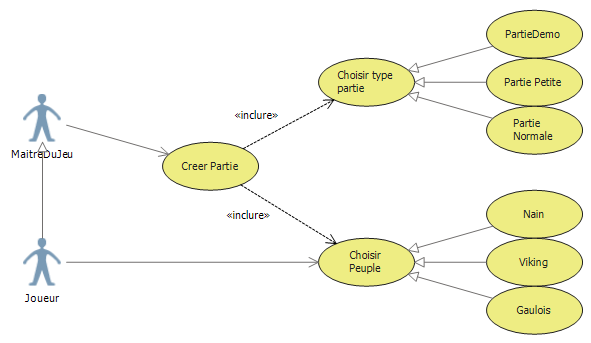
\includegraphics[width=\textwidth]{./images/use_case/DiagUseCaseCreationPartie.png}
                \caption{Diagramme de cas d'utilisation de création d'une partie}
                \label{fig:use_case_creationpartie}
\end{figure}


\begin{figure}[H]
   \centering
   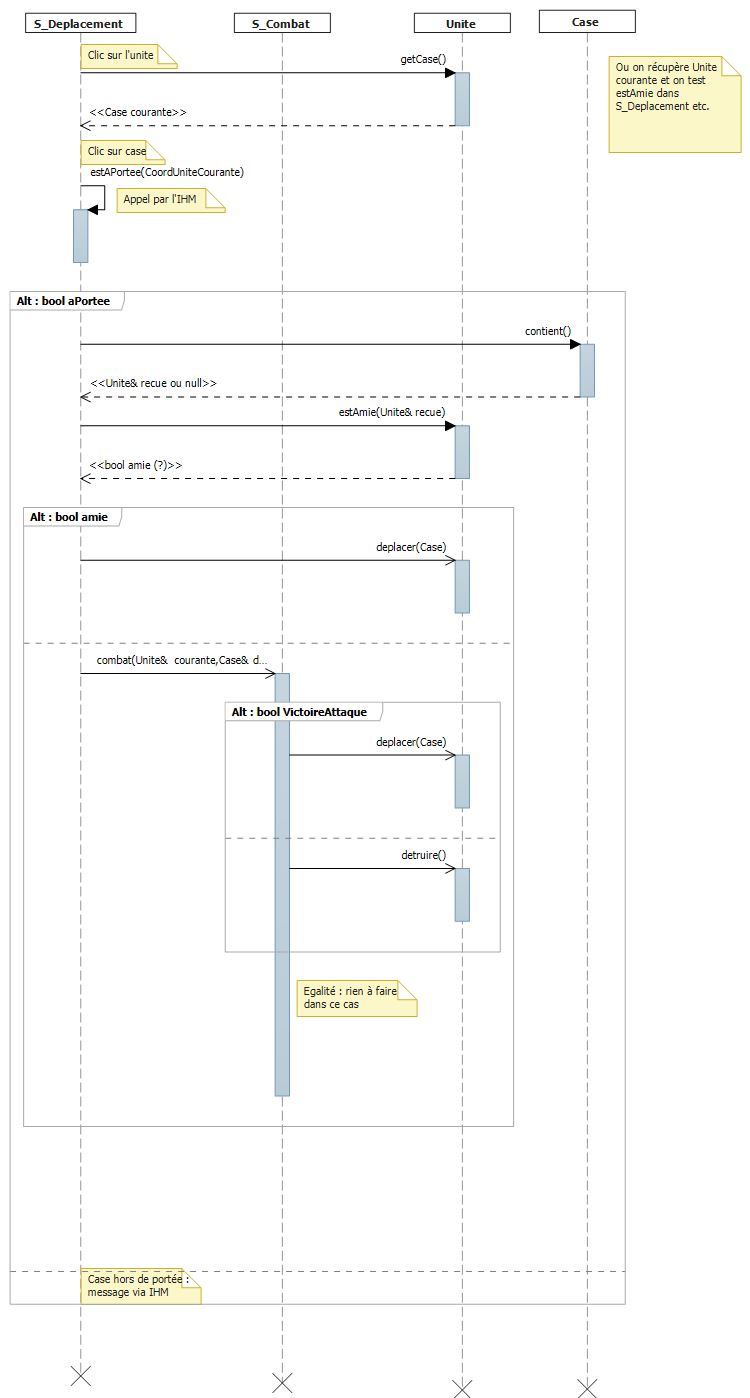
\includegraphics[height=\textwidth,angle =270]{./images/sequence/DiagSeqCreationPartie.png}
                \caption{Diagramme de séquence de création d'une partie}
                \label{fig:sequence_creationpartie}
\end{figure}

\newpage

\subsection{Déroulement d'une partie}

L'état d'une partie à un instant donné dépend de nombreux paramètres : quel est le joueur jouant actuellement ? Y-a-t-il un combat en cours ? Qui gagne ? Le diagramme d'état-transition Figure~\ref{fig:state_transition_deroulementpartie} permet une meilleure visualisation de cet état.

\medskip

	Au cours de son tour de jeu, un joueur doit utiliser toutes ses unités avant de pouvoir accumuler des points. Cette utilisation peut être soit un simple déplacement, soit générer un combat. Lorsqu'il a fini son tour, c'est à l'autre joueur de jouer, si toutefois il reste des tours de jeu.
	
\medskip

	Il y a deux possibilités de terminer une partie : soit un joueur n'a plus d'unité, auquel cas son adversaire à gagner ; soit le nombre maximum de tour a été joué, auquel cas le vainqueur est celui qui a gagné le plus de points au cours de la partie.

\begin{figure}[H]
   \centering
   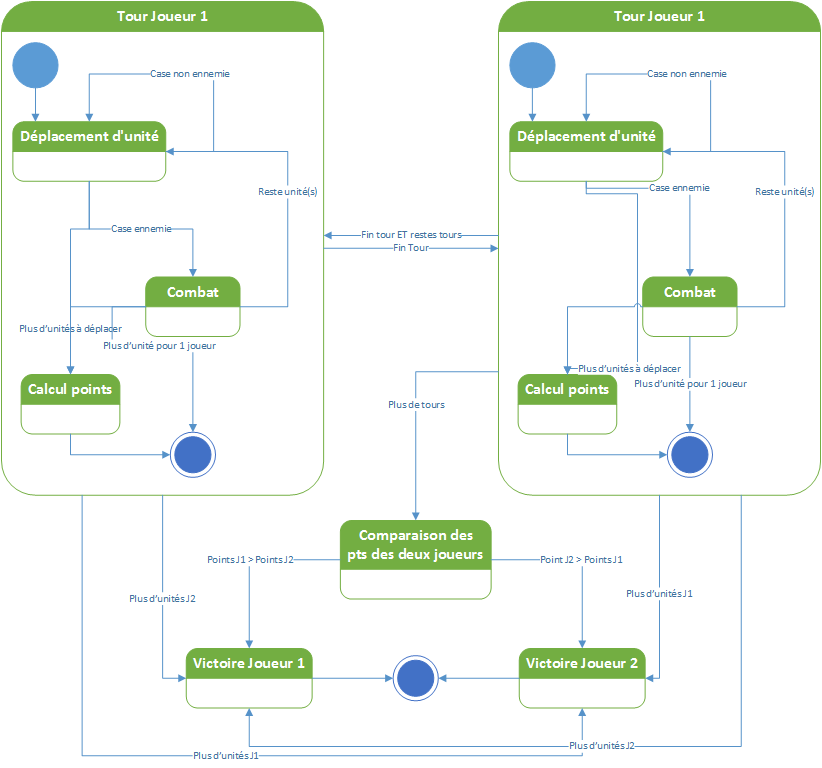
\includegraphics[width=\textwidth]{./images/state_transition/DiagEtatTransitionPartie.png}
                \caption{Diagramme d'état transition du déroulement d'une partie}
                \label{fig:state_transition_deroulementpartie}
\end{figure}

\newpage

\subsection{Déroulement d'un tour}
Le projet est basé sur le vrai jeu de plateau SmallWorld, se déroulant au tour par tour. À chaque tour, le joueur peut effectuer différentes actions (Figure~\ref{fig:use_case_déroulementtour}) pourra utiliser ses unités de la manière dont il veut : attaquer, se déplacer ou ne rien faire. Afin de choisir au mieux ses déplacement, il doit aussi pouvoir analyser les cases de la carte.

\begin{figure}[H]
   \centering
   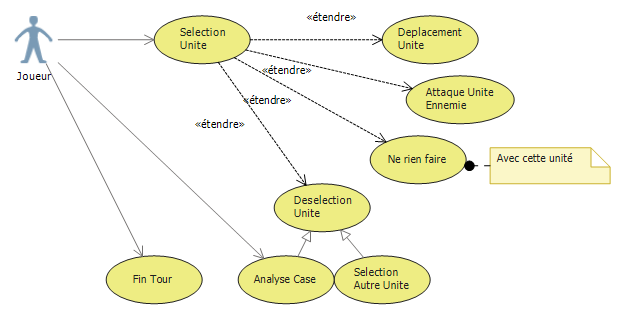
\includegraphics[width=\textwidth]{./images/use_case/DiagUseCaseTour.png}
                \caption{Diagramme de cas d'utilisation de déroulement d'un tour}
                \label{fig:use_case_déroulementtour}
\end{figure}

\newpage

\subsection{Déroulement d'un combat}
L'algorithme des combats étant plus compliqué qu'un simple « si … alors … sinon », il a été nécessaire de réaliser un premier diagramme d'activité (Figure~\ref{fig:activity_déroulementcombat}) afin d'exprimer clairement l'algorithme général, ainsi qu'un deuxième (Figure~\ref{fig:activity_probabilitéscombat}) afin pour celui des calculs de probabilité.

\begin{figure}[H]
    \centering
    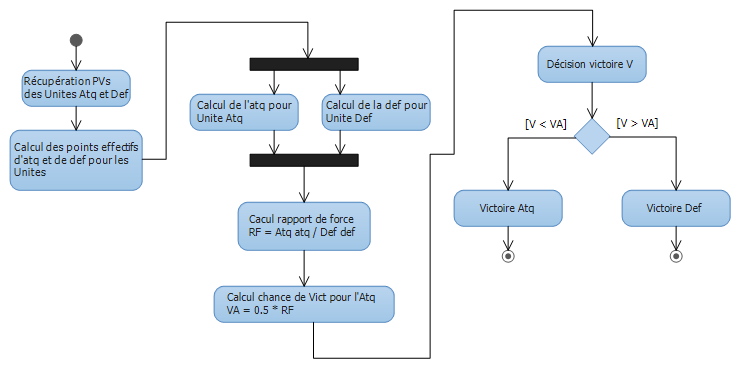
\includegraphics[width=\textwidth]{./images/activity/DiagActivityCombat2.png}
                \caption{Diagramme d'activité du calcul des probabilités d'un combat}
                \label{fig:activity_probabilitéscombat}
\end{figure}

\begin{figure}[H]
    \centering
    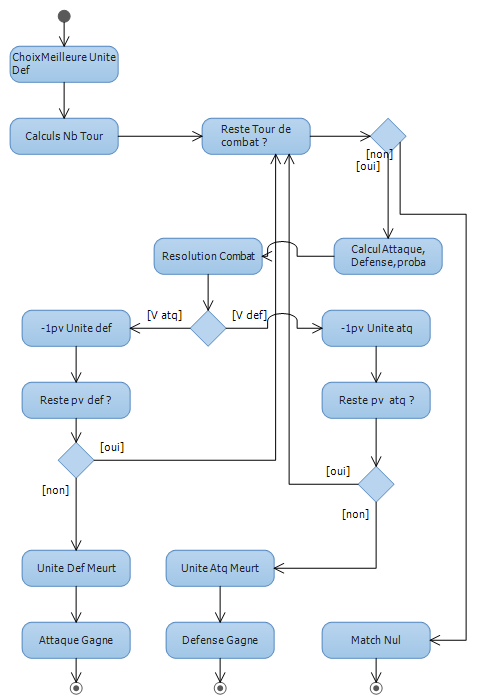
\includegraphics[width=\textwidth]{./images/activity/DiagActivityCombat1.png}
                \caption{Diagramme d'activité d'un combat}
                \label{fig:activity_déroulementcombat}
\end{figure}

\newpage

\subsection{Cycle de vie d'une unité}
L'état d'une unité ne varie qu'en fonction de ses points de vie, son attaque et sa défense propre n'étant jamais modifiées. Le diagramme d'état-transition Figure~\ref{fig:state_transition_cycleviedeunité} montre les différents états possible d'une unité. Un grand état « PV >= 1 » pourrait être fait au lieu des 5 états différents dans le super-état Combat, cependant les points d'attaque et de défense effectifs varient avec les points de vie, aussi faire apparaître chacun de ces états n'est pas dénué d'intérêt.
Le super-état Combat est historique afin de reprendre à chaque nouveau combat en se plaçant sur l'état représentant le nombre de points de vie restant de l'unité à la fin du précédent combat. De plus, la destruction de l'unité s'effectue dès que celle-ci se retrouve dans l'état « Mort », c'est-à-dire qu'elle ne possède plus de point de vie.

\medskip	

De plus, le diagramme de séquence Figure~\ref{fig:sequence_unité} montre la manière dont sera géré une unité au cours d'un tour. Plusieurs cas sont présentés ici, au travers des cadres de séquence : en effet, certaines actions dépendent de l'environnement, comme le fait de vouloir se déplacer vers une case occupée par un ennemi entraîne finalement un combat. Ainsi le message <<bool amie (?) >> est traité selon sa réponse dans les cadres suivants.

\begin{figure}[H]
    \centering
    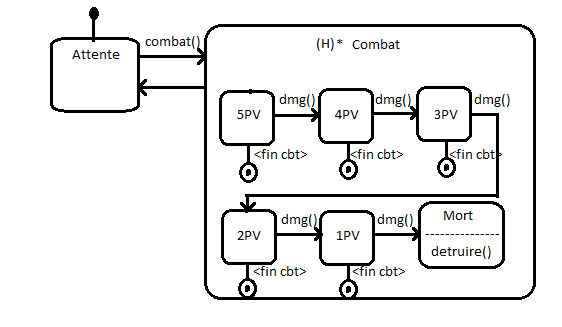
\includegraphics[width=\textwidth]{./images/state_transition/DiagEtatTransitionUnite.png}
                \caption{Diagramme d'état-transitions du cycle de vie d'une unité}
                \label{fig:state_transition_cycleviedeunité}
\end{figure}

\begin{figure}[H]
    \centering
    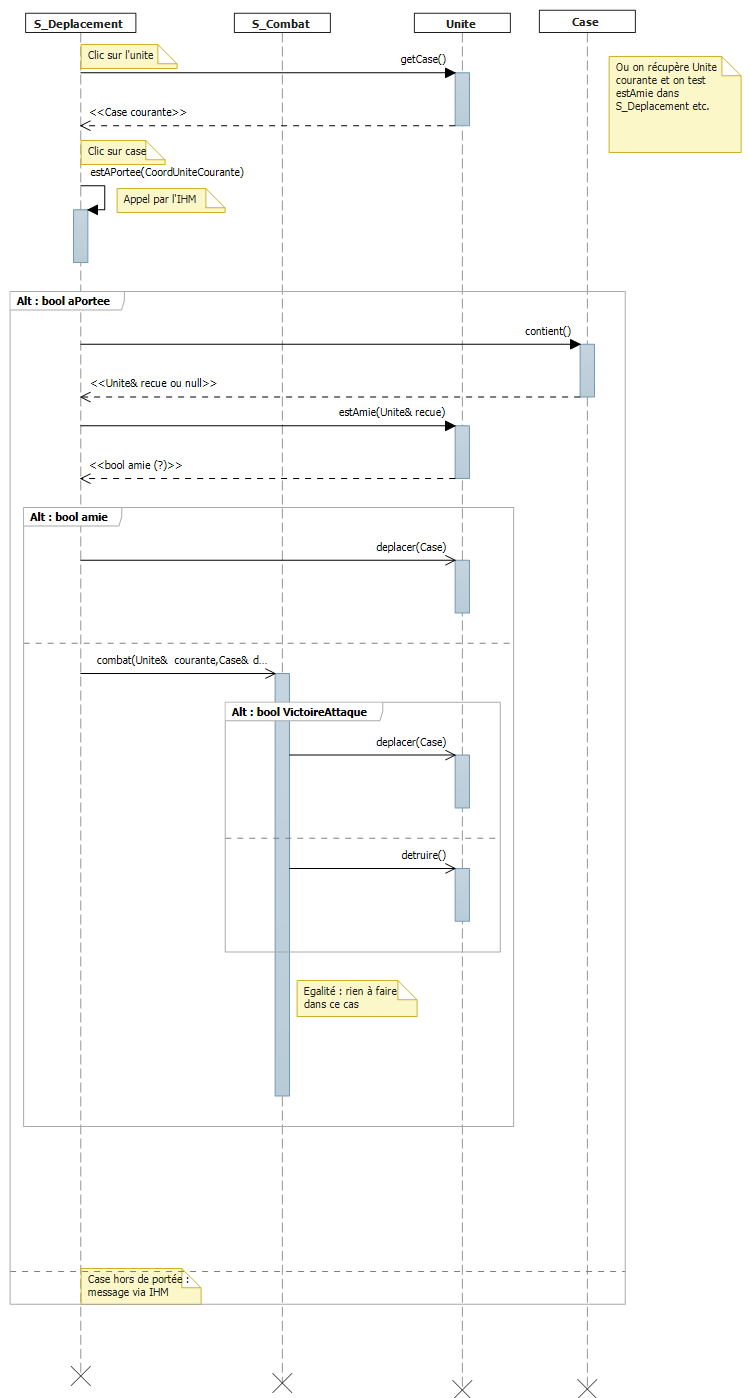
\includegraphics[width=\textwidth]{./images/sequence/DiagSeqUtilisationUnite.png}
                \caption{Diagramme de séquence d'une unité}
                \label{fig:sequence_unité}
\end{figure}

\newpage

\section{Modélisation du diagramme de classe}

Ce diagramme Figure~\ref{fig:class_global} informe la manière dont le jeu sera implémenté en détails : on y retrouve les différentes classes, rangées de sorte à faire ressortir les patrons de conception que nous avons utilisées.

\medskip

	En haut à gauche se trouve le patron de Stratégie Plateau, qui nous servira à construire le plateau et à le remplir en fonction du type de partie choisie : en effet les algorithmes pour remplir une carte n'est pas le même selon sa taille afin d'optimiser le rapport coût-temps de création de celle-ci.

\medskip

	En haut à gauche se situe la partie concernant les cases dont sera composé le plateau. Afin d'optimiser l'utilisation mémoire à la fois à la création et lors de la partie, la patron de poids-mouche est utilisé : Chaque type de case ne sera créé qu'une seul fois par la fabrique de case, puis le plateau ne fera que savoir via une matrice quel le type d'une case. Ainsi chaque case ne sera pas très lourde.
Par ailleurs, puisque projet comporté originalement des bonus sur certaines cases, le choix avait été fait de réaliser également un poids-mouchage de ceux-ci, tout en les considérant que des décorations des cases. Cette implémentation sera réalisée si possible selon l'avancement du projet, mais nous avons décidé de garder la trace de notre réflexion à ce sujet.

\medskip

	En bas à droit se situe tout ce qui constitue le jeu en dehors des classes de modélisation du jeu « physique ». On y retrouve un singleton Combat qui sera responsable de la résolution des combats, ceux-ci se déroulant un par un et toujours de la même manière. Il contiendra entre autre l'algorithme de résolution des combats vu précédemment.

\medskip

Nous retrouvons également le patron de montage afin de créer une partie. Il n'est pas nécessaire de créer une classe pour chacun des types de partie : le seul changement se situant à la création du plateau, le monteur appellera donnera simplement la bonne stratégie au plateau.

\medskip

La classe joueur est également présente afin de compter les points, connaître l'appartenance des unités etc.

\medskip

	En bas à droite se situe la fabrique d'unité selon le peuple choisi. Il n'est pas nécessaire de créer une classe fabrique : chaque peuple ne construisant qu'un seul type d'unité, et surtout ces unités n'étant créée qu'une seule fois au début de la partie, la méthode de créations de celles-ci peut être située directement dans la classe peuple.

\medskip

	La gestion de la vue n'est pas visualisable ici car il existe une méthode spécifique au C\# qui n'est pas représentable sur un diagramme de classe.


\begin{figure}[H]
    \centering
    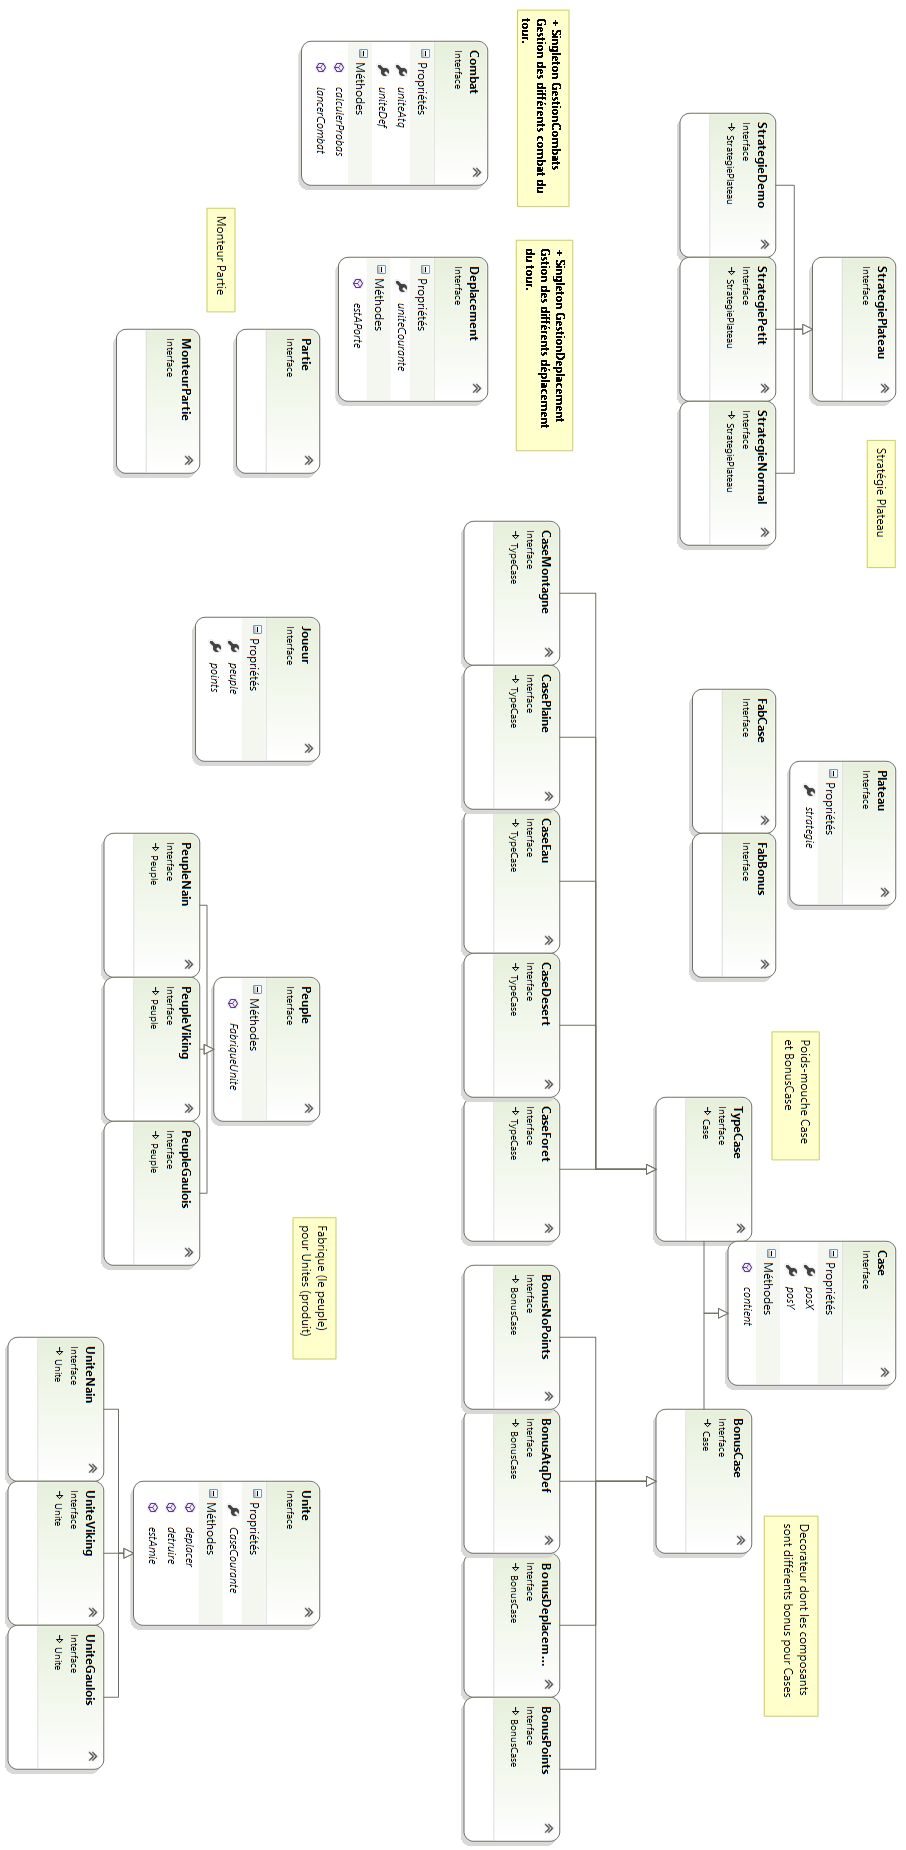
\includegraphics[width=\textwidth, height=\textheight]{./images/class/interfacesPortrait.png}
                \caption{Diagramme de classes global}
                \label{fig:class_global}
\end{figure}


\newpage

\section*{Conclusion}
\addcontentsline{toc}{section}{Conclusion}

L'objectif du projet d'analyse, conception et POO de quatrième année informatique est la création d'un jeu vidéo basé sur le jeu de plateau Small World, pour mettre en pratique et appliquer les concepts vu en cours de modélisation et POO.

\medskip

Après cette phase de conception nous ayant permis de définir l'architecture de l'application ainsi que son fonctionnement, nous devons réaliser l'implémentation de ses différents composants tout en les testant au fur et à mesure.

\newpage
\listoffigures


\end{document}